\documentclass[12pt, letterpaper]{article}
\usepackage{bbold}
\usepackage{indentfirst}
\usepackage{amsmath, amssymb}
\usepackage[T1]{fontenc}
\usepackage[utf8]{inputenc}
\usepackage{physics}
\usepackage{tensor}
\usepackage{braket}
\usepackage{graphics}
\usepackage{grffile}
\usepackage[export]{adjustbox}
\usepackage{svg}
\usepackage{caption}
\usepackage{subcaption}
\usepackage{authblk}
%\usepackage[a4paper, total={6in, 8in}]{geometry}

\graphicspath{ {/home/nooremf/Project/Code/Thesis/}}
\newcommand*{\1}{\hspace{1pt}}
\title{Magnetic and Optical Properies of  LiNbO3 Type InCoO3 and InFeO3 perovskite materials.}
%\title{\color{blue} \Huge{ DISCUSSION ON THE HARD-SPHERE THEORY}}

%\author{ COURCE TITLE : HONOURS PROJECT \\ COURCE CODE : TP-407 \\ \textbf{SUBMITTED BY} \\ [5PT] \Large MD. ROMIJ UDDIN \\ \Large ROLL : SH-098-035 \\ \Large REGISTRATION NUMBER : 2016-614-721 \\ \Large  ACADEMIC YEAR :  2019-20 \\ \Large  SESSION : 2016-17
%\\ [10pt] 
%\includegraphics[width=0.5\textheight]{du} \\ [10pt] \Large DEPARTMENT OF THEORETICAL PHYSICS \\ UNIVERSITY OF DHAKA 
%}

\author{Noor E Mustafa Ferdous}


\date{20/3/2022}

\begin{document}
    \maketitle
    %\section*{Magnetic and Optical Properies of  LiNbO3 Type InCoO3 and InFeO3 perovskite materials.}
    \subsection*{Abstract}
    Metal oxide perovskites are increasingly popular for magnetic and optoelectronic applications in industrial purposes. In this study, structural magnetic and 
    optical properties of InCoO3, and InFeO3 were unearthed using the first principles of density functional theory. These materials exhibit semiconducting behavior 
    with indirect bandgap energy. The high absorption coefficient, low reflectivity, and high optical conductivity make them suitable for photovoltaic and other 
    optoelectronic and memory device applications. Among them, InFeO3 is more favorable for magnetic and optical applications.

    \subsection*{Introduction}
    In a quest for nanoparticles, solar cells, and enhanced optical and magnetic properties, perovskite materials suit flawlessly in that range. Perovskite materials 
    contain properties like tunable bandgap, long charge diffusion length, good charge carrier mobility, low carrier recombination rate, high dielectric constant. 
    They have high efficiency in photoconductor-based X-ray detectors, spectroscopy, acoustic wave signal processing, and image storage device. These materials are 
    the class of material that bears the chemical structure of $ABO_{3}$.
    
    \begin{adjustbox}{center,caption={Cubic Structure of InCoO3 and InFeO3},label={somelabel},nofloat=figure,vspace=\bigskipamount}
        \includegraphics[width=0.7\textwidth]{InFeO3}
        \includegraphics[width=0.7\textwidth]{InFeO3}
    \end{adjustbox}
    
    In this type of material, O is oxygen with (-2) ionic valence anion, and A and B metal 
    cations give (+6) valence ion combined. Perovskite material family has numerous types of oxide form like transition metal oxides with the general formula of ABO3.
    One perovskite material is LiNbO3. For that, we took LiNbO3-like material InCoO3, InFeO3 and sampled magnetic and optical properties with DFT calculations. 
    
    \subsection*{Computaion Method}
    For computing the magnetic and optical properties of InFeO3 and InCoO3, we execute Density Functional Theory (DFT) simulations by  Vienna ab initio Simulation 
    Package (VASP). The unit cells of InCoO3 and InFeO3 in the cubic form are shown in Fig. 1, which we explored further. First, we perform structural relaxation. 
    Then we execute static calculation for density of states, band, and optical properties of chosen materials. 
    
%    \begin{figure}[h]
%
%        \begin{subfigure}{0.5\textwidth}
%        \includegraphics[width=0.4\paperwidth, height=6cm]{InFeO3}
%        \caption{Caption1}
%        \label{fig:subim1}
 %       \end{subfigure}
 %       \begin{subfigure}{0.5\textwidth}
 %       \includegraphics[width=0.4\paperwidth, height=6cm]{InCoO3}
 %       \end{subfigure}
            
    %\end{figure} 
    %\begin{figure}[H]
    %\centering
    %\includegraphics[scale=.3]{InFeO3}
    %\includegraphics[scale=.3]{InCoO3}
    %\end{figure}

    \begin{adjustbox}{center,caption={Band Structure Of InCoO3 and InFeO3},label={somelabel},nofloat=figure,vspace=\bigskipamount}
        \includegraphics[width=0.7\textwidth]{bandCo}
        \includegraphics[width=0.7\textwidth]{bandFe}
    \end{adjustbox}

    \subsection*{Results}
    InFeO3 and InCoO3 are cubic structures under the space group of Pm3m (no. 221). We visualize the structures in VESTA (3D Visualization for Electronic and 
    Structural Analysis). The unit cell of InCoO3 and InFeO3 constitutes five atoms (shown in Fig. 1). Fe or Co atoms hold the corner positions of the cubes (Wyckoff 
    site (0,0,0)), In situated in the crystal's body-centered positions (Wyckoff site(0.5,0.5,0.5)). O occupies face-centered positions (Wyckoff site (0.5,0.5,0)). 
    The electronic band structures and density of states(DOS) of relaxed InCoO3 and InFeO3 structures through PBE functional considering the GGA approximation. 
    Band structures of InCoO3 and InFeO3 are shown in Fig. 2.  


    
    Zero-point energy is Fermi energy.Two structures show indirect bandgap and the range of the bandgap 
    energy resembles that both the structures are metallic in nature. The outcome of the bandgaps and band structures of the examined materials confirm their wonder
    for photothermal, photovoltaic, and optoelectronic applications. InCoO3 and InFeO3 show the same bandgap. The density of states of atoms is shown in Fig. 3.
    
    \begin{adjustbox}{center,caption={Density of States Of InCoO3 and InFeO3},label={somelabel},nofloat=figure,vspace=\bigskipamount,}
        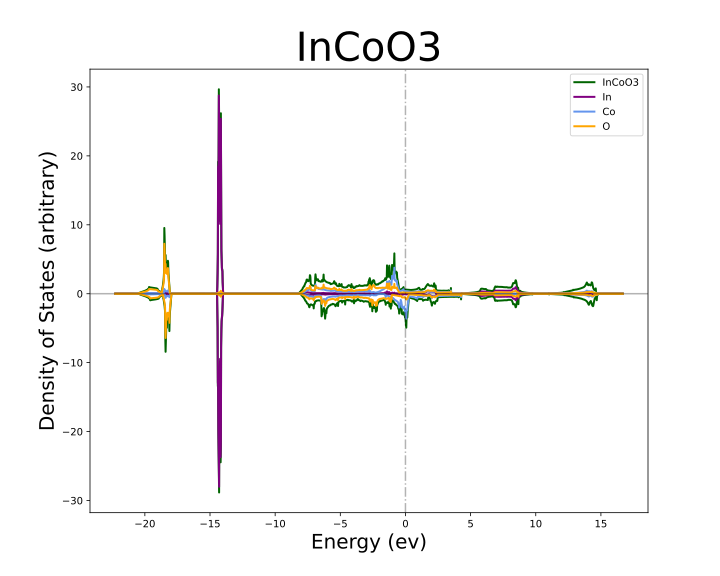
\includegraphics[width=0.7\textwidth]{DosInCoO3}
        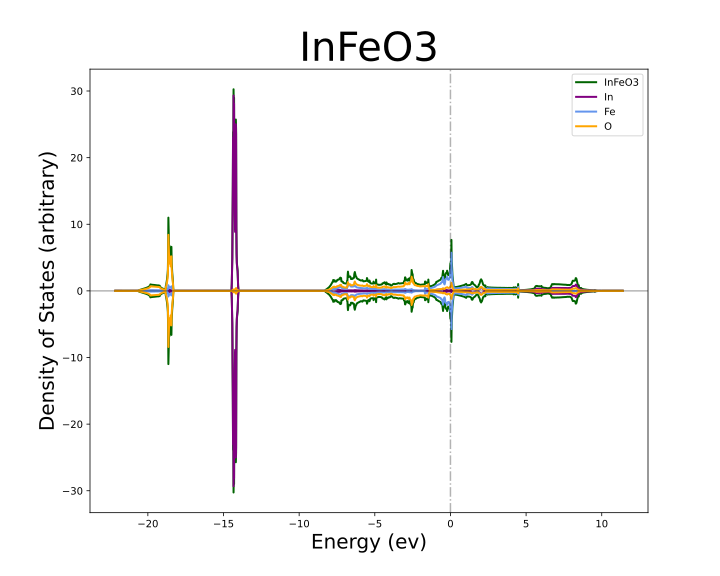
\includegraphics[width=0.7\textwidth]{DosInFeO3}
    \end{adjustbox}
    
    The orbital projected density of states indicates at the Fermi level, the p-orbital of Co and Fe atom is the main benefactor. The optical properties of a 
    material rely on many parts. Such as absorption spectra, concerning light energy and wavelength, reflectivity, refractivity index, dielectric constants, and 
    optical conductivity. We examined these properties with InCoO3 and InFeO3.  The optical absorption coefficient indicates how much light penetrates the substance 
    before being absorbed by the material. This is a piece of important knowledge for solar-energy conversion efficiency for practical application. In Fig. 4 energy 
    and wavelength-dependent absorption profiles are demonstrated.
    
    \begin{adjustbox}{center,caption={Absorption Of InCoO3 and InFeO3},label={somelabel},nofloat=figure,vspace=\bigskipamount,}
        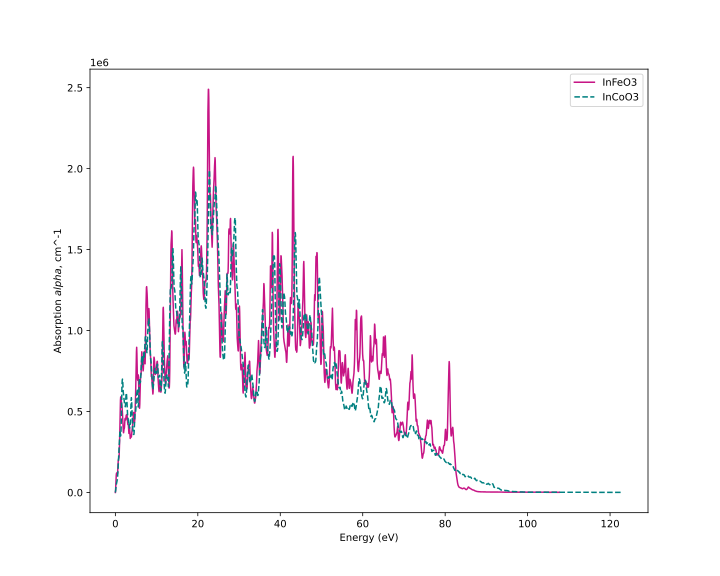
\includegraphics[width=0.8\textwidth]{Absorptioneng}
    \end{adjustbox}
    
    Reflectivity is an optical property to understand the surface nature of the material. It defines 
    how much energy reflects from incident energy on the surface. Fig 5 represents the optical reflectivity of InCoO3 and InFeO3. 
    
    \begin{adjustbox}{center,caption={Reflectivity Of InCoO3 and InFeO3},label={somelabel},nofloat=figure,vspace=\bigskipamount,}
        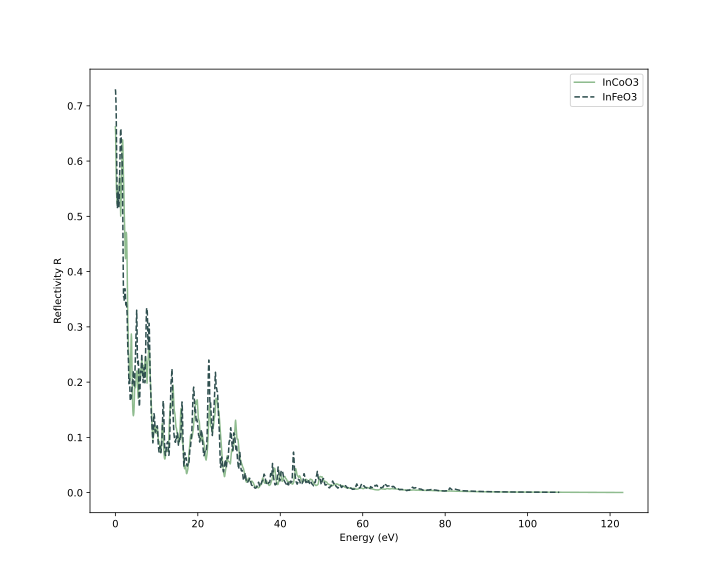
\includegraphics[width=0.8\textwidth]{refleceng}
    \end{adjustbox}
    
    The dielectric constant values are used for determining how well optoelectronic devices work, defined as the response of a material to incident light energy. Higher dielectric values at a lower 
    charge carrier recombination rate are deep in improving the optoelectronic device performance. The optical conductivity of a material specifies the electric 
    conductivity of a photon from electromagnetic absorption. Fig 6 shows the dielectric constants of InCoO3 and InFeO3. Fig 7 shows us optical conductivity between
    InCoO3 and InFeO3.

    \begin{adjustbox}{center, caption={Dielectric constants of InCoO3 and InFeO3},label={somelabel},nofloat=figure,}
        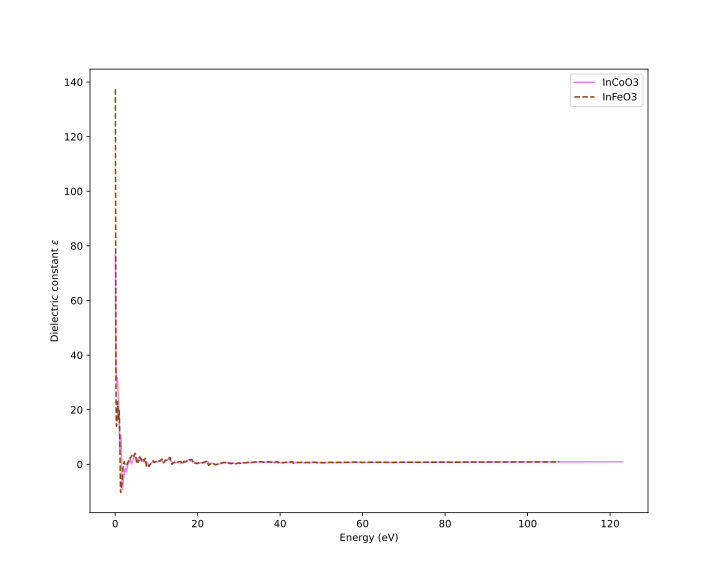
\includegraphics[width=0.7\textwidth]{dieleceng}
        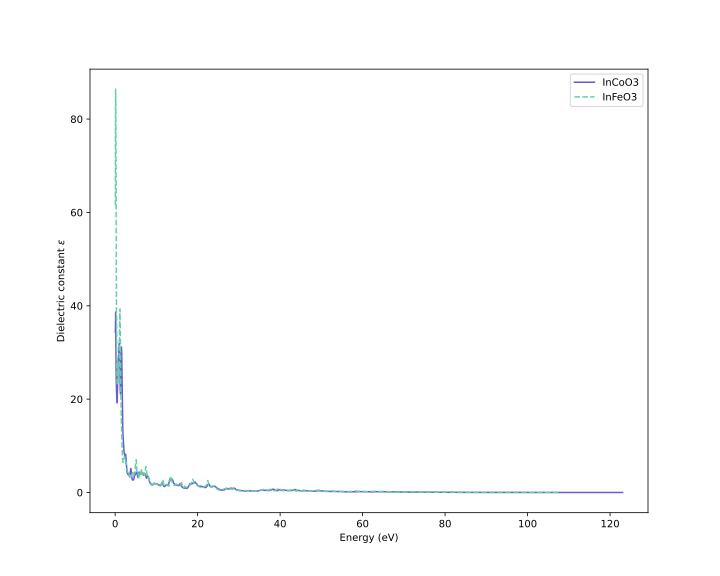
\includegraphics[width=0.7\textwidth]{dielecimageng}
    \end{adjustbox}
    

    \begin{adjustbox}{center,caption={Optical Conductivity of InCoO3 and InFeO3},label={somelabel},nofloat=figure,}
        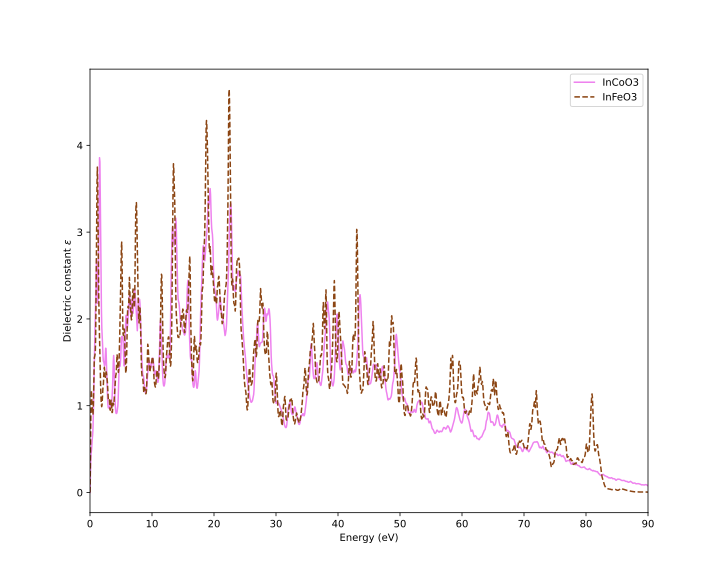
\includegraphics[width=0.7\textwidth]{opcondrealev}
        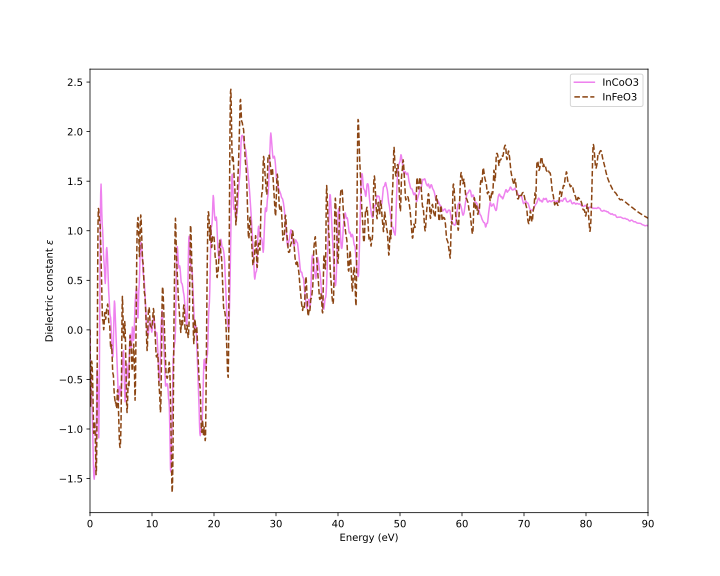
\includegraphics[width=0.7\textwidth]{opcondimagev}
    \end{adjustbox}

    \subsection*{Conclusion}
    We performed a study on  InCoO3 and InFeO3 perovskite cubic materials using  DFT simulations for their structural, optical, and dielectric properties. InCoO3
    and InFeO3 structures show identical indirect bandgap while InFeo3 shows more magnetic than InCoO3. Fe is a better contender than Co for optical absorption 
    and optical conductivity. Both the material can be an excellent choice for various photovoltaic applications, memory devices, and more.

    
\end{document}